\documentclass[11pt,a4paper]{article}
\usepackage[T1]{fontenc}
\usepackage[utf8]{inputenc}
\usepackage[margin=22mm,headheight=15pt,headsep=9mm,footskip=12mm]{geometry}
\usepackage{tgpagella}
\usepackage[scaled=.92]{tgheros}
\usepackage{inconsolata}
\usepackage{xcolor}
\usepackage{tikz}
\usetikzlibrary{positioning,arrows.meta,shapes.geometric,fit,calc,shadows}
\usepackage{tcolorbox}
\tcbuselibrary{skins,breakable}
\usepackage{booktabs}
\usepackage{array}
\usepackage{enumitem}
\usepackage{fancyhdr}
\usepackage{titlesec}
\usepackage{listings}
\usepackage{hyperref}

% One palette, shared by text, cards, tables, links, and diagrams.
\definecolor{Primary}{HTML}{18364A}
\definecolor{Accent}{HTML}{00877E}
\definecolor{Amber}{HTML}{B77A16}
\definecolor{Ink}{HTML}{35434F}
\definecolor{Muted}{HTML}{647887}
\definecolor{Soft}{HTML}{F2F6F8}
\definecolor{Paper}{HTML}{FFFFFF}

\hypersetup{colorlinks=true,linkcolor=Accent,urlcolor=Accent,
  pdftitle={Pilot / Phase 1 / Foundation},pdfauthor={Pilot},
  pdfsubject={A compact guide to the implemented agent foundation},
  bookmarksopen=true,bookmarksnumbered=false}
\urlstyle{tt}
\linespread{1.15}
\setlength{\parindent}{0pt}
\setlength{\parskip}{6pt}
\setlength{\emergencystretch}{2em}
\setcounter{tocdepth}{1}
\renewcommand{\contentsname}{Your reading map}
\renewcommand{\arraystretch}{1.5}
\setlength{\tabcolsep}{4pt}
\setlist{nosep,leftmargin=*,itemsep=5pt,topsep=4pt}
\titleformat{\section}{\sffamily\LARGE\bfseries\color{Primary}}{}{0pt}{}
\titlespacing*{\section}{0pt}{0pt}{12pt}
\pagestyle{fancy}
\fancyhf{}
\fancyhead[L]{\sffamily\small\color{Muted}PILOT\quad /\quad PHASE 01}
\fancyhead[R]{\sffamily\small\color{Primary}FOUNDATION}
\fancyfoot[L]{\sffamily\scriptsize\color{Muted}Agent engineering / concept notes}
\fancyfoot[R]{\sffamily\small\color{Primary}\thepage}
\renewcommand{\headrulewidth}{.4pt}
\renewcommand{\footrulewidth}{0pt}
\renewcommand{\headrule}{\hbox to\headwidth{\color{Primary!15}\leaders\hrule height .4pt\hfill}}

% Reusable card and diagram styles are defined only here.
\tcbset{
  conceptbox/.style={enhanced,breakable,colback=Paper,colframe=Primary!18,
    coltext=Ink,boxrule=.45pt,arc=3mm,left=4mm,right=4mm,top=3mm,bottom=3mm,
    borderline west={2pt}{0pt}{Accent},
    colbacktitle=Soft,coltitle=Primary,fonttitle=\sffamily\bfseries,
    attach boxed title to top left={xshift=4mm,yshift=-2mm},
    boxed title style={boxrule=0pt,arc=1mm,left=2mm,right=2mm},
    before skip=3mm,after skip=3mm},
  analogybox/.style={enhanced,colback=Accent!6,colframe=Accent!20,
    coltext=Ink,boxrule=.4pt,arc=2mm,left=4mm,right=4mm,top=2mm,bottom=2mm,
    fontupper=\small,before skip=3mm,after skip=3mm},
  warnbox/.style={enhanced,colback=Amber!8,colframe=Amber!35,
    coltext=Ink,boxrule=.4pt,arc=2mm,left=4mm,right=4mm,top=3mm,bottom=3mm,
    borderline west={2pt}{0pt}{Amber},fontupper=\small,
    before skip=3mm,after skip=3mm},
  interviewbox/.style={enhanced,colback=Primary!4,colframe=Primary!18,
    coltext=Ink,coltitle=Primary,colbacktitle=Primary!7,
    fonttitle=\sffamily\bfseries,boxrule=.4pt,arc=2mm,
    left=4mm,right=4mm,top=3mm,bottom=3mm,
    before skip=3mm,after skip=3mm}
}
\tikzset{
  block/.style={rectangle,rounded corners=3pt,draw=Primary!25,fill=Soft,
    text=Ink,font=\sffamily\small,align=center,text width=3cm,
    minimum height=11mm,inner sep=5pt},
  decision/.style={diamond,aspect=2,draw=Accent!50,fill=Accent!7,
    text=Ink,font=\sffamily\small,align=center,text width=19mm,inner sep=2pt},
  store/.style={cylinder,shape border rotate=90,aspect=.2,
    draw=Primary!30,fill=Primary!5,text=Ink,font=\sffamily\small,
    align=center,text width=3cm,minimum height=14mm,inner sep=5pt},
  arrow/.style={-{Latex[length=2.2mm,width=1.6mm]},thick,draw=Accent},
  every label/.style={font=\sffamily\scriptsize,text=Muted}
}
\lstset{basicstyle=\ttfamily\small\color{Ink},keywordstyle=\color{Primary},
  commentstyle=\color{Muted},stringstyle=\color{Accent},
  backgroundcolor=\color{Soft},frame=none,breaklines=true,
  columns=fullflexible,keepspaces=true,showstringspaces=false}

\newcommand{\refcode}[2]{{\footnotesize\color{Muted}\path{#1}:\allowbreak\ \texttt{#2}}}
\newcommand{\tagline}[1]{{\sffamily\scriptsize\bfseries\color{Accent}#1}\par}
\newcommand{\pageheading}[2]{%
  \clearpage\phantomsection\addcontentsline{toc}{section}{#2}%
  \tagline{#1}\section*{#2}}
\newcommand{\card}[5]{%
  \begin{tcolorbox}[conceptbox,title={#1},height=55mm]
    \textbf{What}\enspace #2\par
    \textbf{Why}\enspace #3\par
    \vfill\textbf{In our code}\par\refcode{#4}{#5}
  \end{tcolorbox}}
\newcommand{\pair}[2]{%
  \begin{minipage}[t]{.485\linewidth}#1\end{minipage}\hfill
  \begin{minipage}[t]{.485\linewidth}#2\end{minipage}\par}
\newcommand{\captionline}[1]{{\footnotesize\color{Muted}#1}\par}
\newcommand{\term}[2]{\textbf{#1}\enspace #2\par}

\begin{document}
\color{Ink}

% PAGE 1 -- overview. Architecture diagram: 8 nodes.
\phantomsection\addcontentsline{toc}{section}{Overview: the whole foundation}
\tagline{ENGINEERING NOTES / 01}
{\sffamily\fontsize{43}{47}\selectfont\bfseries\color{Primary}Foundation}\par
{\Large A small agent. Explicit control.}\par
\vspace{8mm}
\begin{center}
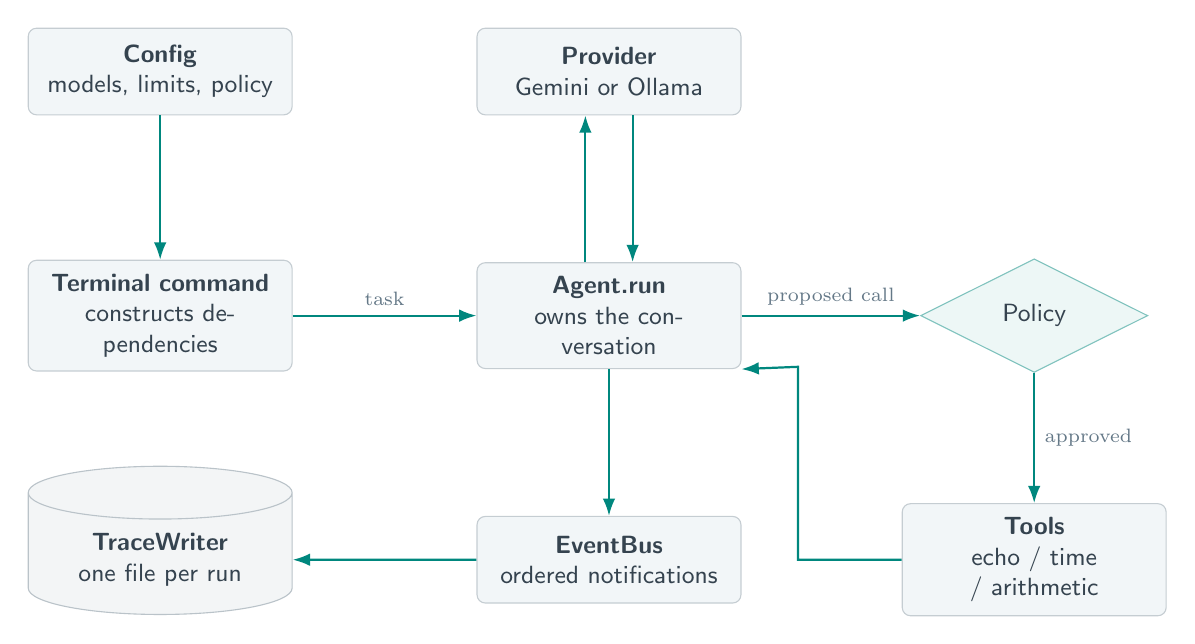
\begin{tikzpicture}
  \node[block] (config) at (0,6.2) {\textbf{Config}\\models, limits, policy};
  \node[block] (cli) at (0,3.1) {\textbf{Terminal command}\\constructs dependencies};
  \node[block] (agent) at (5.7,3.1) {\textbf{Agent.run}\\owns the conversation};
  \node[block] (provider) at (5.7,6.2) {\textbf{Provider}\\Gemini or Ollama};
  \node[decision] (policy) at (11.1,3.1) {Policy};
  \node[block] (tools) at (11.1,0) {\textbf{Tools}\\echo / time / arithmetic};
  \node[block] (bus) at (5.7,0) {\textbf{EventBus}\\ordered notifications};
  \node[store] (trace) at (0,0) {\textbf{TraceWriter}\\one file per run};
  \draw[arrow] (config)--(cli);
  \draw[arrow] (cli)--node[above,font=\scriptsize,text=Muted]{task}(agent);
  \draw[arrow] ([xshift=-3mm]agent.north)--([xshift=-3mm]provider.south);
  \draw[arrow] ([xshift=3mm]provider.south)--([xshift=3mm]agent.north);
  \draw[arrow] (agent)--node[above,font=\scriptsize,text=Muted]{proposed call}(policy);
  \draw[arrow] (policy)--node[right,font=\scriptsize,text=Muted]{approved}(tools);
  \draw[arrow] (tools.west)--(8.1,0)--(8.1,2.45)--(agent.south east);
  \draw[arrow] (agent)--(bus);
  \draw[arrow] (bus)--(trace);
\end{tikzpicture}
\end{center}
\vspace{7mm}
\begin{tcolorbox}[conceptbox,title={What we built and why}]
  An agent turns model suggestions into controlled actions.\\
  Two providers, three demo tools, approval rules, and run records.\\
  A testable foundation for more powerful capabilities later.
\end{tcolorbox}
\captionline{Source map: \path{src/pilot/agent/loop.py}: \texttt{Agent.run};
  \path{src/pilot/cli.py}: \texttt{create\_app}.}

% PAGE 2 -- clickable contents.
\clearpage\tagline{START HERE}\tableofcontents
\vfill
\begin{tcolorbox}[analogybox]
  \textbf{Reading route}\quad Scan the diagrams, read the cards, then explain the interview answers aloud.
\end{tcolorbox}
\begin{tcolorbox}[warnbox]
  \textbf{Evidence boundary}\quad The walkthrough uses an existing offline test.
  It demonstrates our control flow, not live-provider acceptance.
\end{tcolorbox}

% PAGE 3 -- concepts 1--2. Loop diagram: 8 nodes.
\pageheading{CONCEPTS / MODEL + CONTROL}{A conversation with a stopping rule}
\pair{
  \card{01 / Stateless API}{An LLM is a language model. Its API, a calling contract, receives the context again on each request.}{Roles separate system instructions, user tasks, assistant replies, and tool results.}{src/pilot/providers/base.py}{Message}
}{
  \card{02 / Loop + limits}{The agent repeats think, act, observe. A plain answer finishes.}{Step limits bound provider calls; token limits bound reported text units. Checks happen after each response.}{src/pilot/agent/loop.py}{Agent.run}
}
\vspace{7mm}
\begin{center}
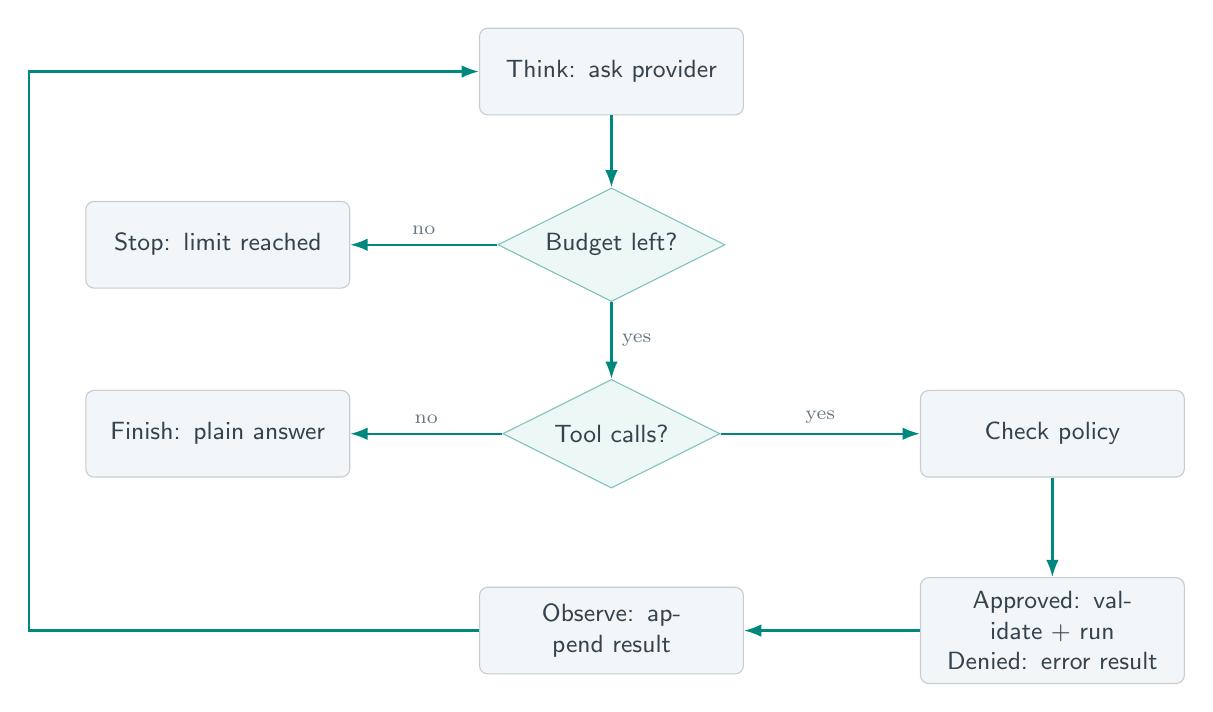
\begin{tikzpicture}
  \node[block] (think) at (0,7.5) {Think: ask provider};
  \node[decision] (budget) at (0,5.3) {Budget left?};
  \node[decision] (call) at (0,2.9) {Tool calls?};
  \node[block] (policy) at (5.6,2.9) {Check policy};
  \node[block] (run) at (5.6,.4) {Approved: validate + run\\Denied: error result};
  \node[block] (observe) at (0,.4) {Observe: append result};
  \node[block] (finish) at (-5,2.9) {Finish: plain answer};
  \node[block] (limit) at (-5,5.3) {Stop: limit reached};
  \draw[arrow] (think)--(budget);
  \draw[arrow] (budget)--node[right,font=\scriptsize,text=Muted]{yes}(call);
  \draw[arrow] (budget)--node[above,font=\scriptsize,text=Muted]{no}(limit);
  \draw[arrow] (call)--node[above,font=\scriptsize,text=Muted]{no}(finish);
  \draw[arrow] (call)--node[above,font=\scriptsize,text=Muted]{yes}(policy);
  \draw[arrow] (policy)--(run);
  \draw[arrow] (run)--(observe);
  \draw[arrow] (observe.west)--(-7.4,.4)--(-7.4,7.5)--(think.west);
\end{tikzpicture}
\end{center}
\begin{tcolorbox}[warnbox]
  A response can overshoot the token budget. At exhaustion, none of its tool calls executes.
\end{tcolorbox}
\captionline{Step exhaustion is checked before the next provider call. Internal HTTP retries do not add agent steps.}

% PAGE 4 -- concepts 3--4. Provider diagram: 6 nodes.
\pageheading{CONCEPTS / BOUNDARIES}{One interface, independent instances}
\pair{
  \card{03 / Provider abstraction}{An interface specifies required behavior. An adapter translates a vendor's format into our shared messages.}{The loop calls a Python Protocol, an interface contract, rather than inspecting vendor fields.}{src/pilot/providers/base.py}{LLMProvider}
}{
  \card{04 / Dependency injection}{Dependencies are required collaborators. Injection supplies them explicitly.}{Each agent can own separate tools, provider, policy, bus, and prompt; conversations stay local to each run.}{src/pilot/agent/loop.py}{Agent.\_\_init\_\_}
}
\vspace{10mm}
\begin{center}
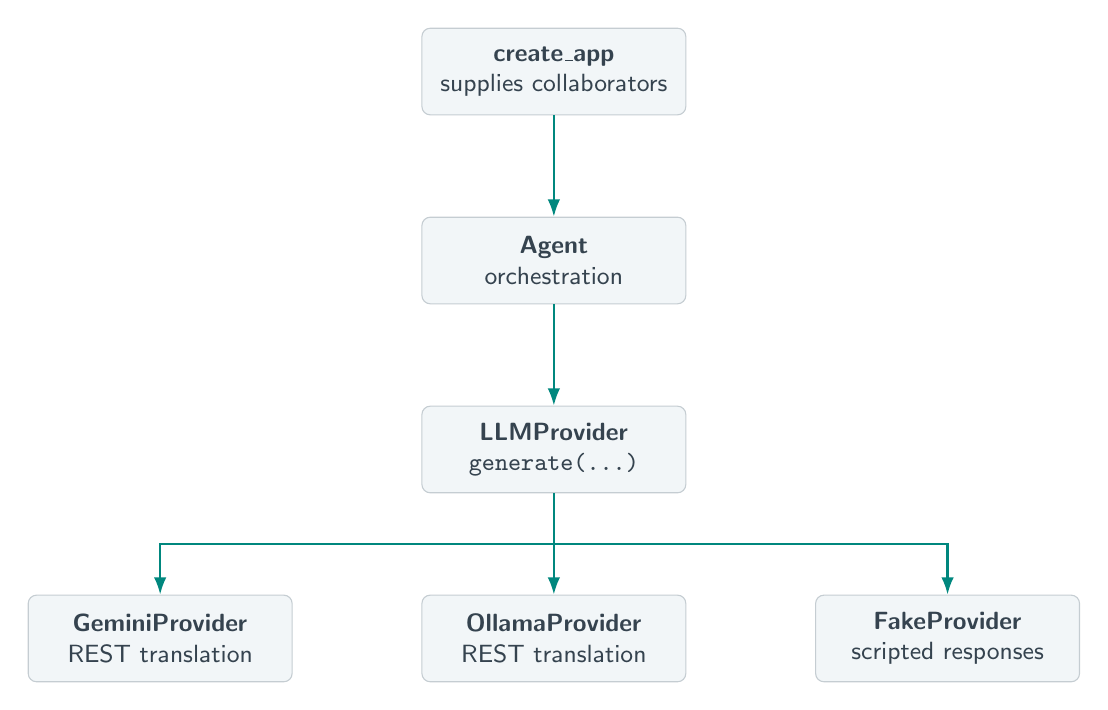
\begin{tikzpicture}
  \node[block] (construct) at (0,7.2) {\textbf{create\_app}\\supplies collaborators};
  \node[block] (agent) at (0,4.8) {\textbf{Agent}\\orchestration};
  \node[block] (interface) at (0,2.4) {\textbf{LLMProvider}\\\texttt{generate(...)} };
  \node[block] (gemini) at (-5,0) {\textbf{GeminiProvider}\\REST translation};
  \node[block] (ollama) at (0,0) {\textbf{OllamaProvider}\\REST translation};
  \node[block] (fake) at (5,0) {\textbf{FakeProvider}\\scripted responses};
  \draw[arrow] (construct)--(agent);
  \draw[arrow] (agent)--(interface);
  \draw[arrow] (interface.south)--(0,1.2)-|(gemini.north);
  \draw[arrow] (interface)--(ollama);
  \draw[arrow] (interface.south)--(0,1.2)-|(fake.north);
\end{tikzpicture}
\end{center}
\begin{tcolorbox}[analogybox]
  \textbf{Analogy}\quad The same socket accepts different adapters; separate desks keep separate case folders.
\end{tcolorbox}
\captionline{REST here uses direct HTTP web requests.
  \refcode{src/pilot/providers/__init__.py}{create\_provider} selects the implementation.}

% PAGE 5 -- concepts 5--6. Permission diagram: 8 nodes.
\pageheading{CONCEPTS / ACTIONS}{A request is not permission}
\pair{
  \card{05 / Tools + schemas}{A tool call names an action and arguments. JSON is structured text; JSON Schema describes allowed shapes.}{Pydantic validates arguments. The registry returns structured errors instead of crashing.}{src/pilot/tools/registry.py}{ToolRegistry.execute}
}{
  \card{06 / Policy + approval}{Policy resolves allow, ask, or deny. Human-in-the-loop means a person decides at the approval point.}{Ask by default prevents silent execution. Least privilege means granting only necessary access.}{src/pilot/permissions.py}{PolicyEngine.decide}
}
\vspace{7mm}
\begin{center}
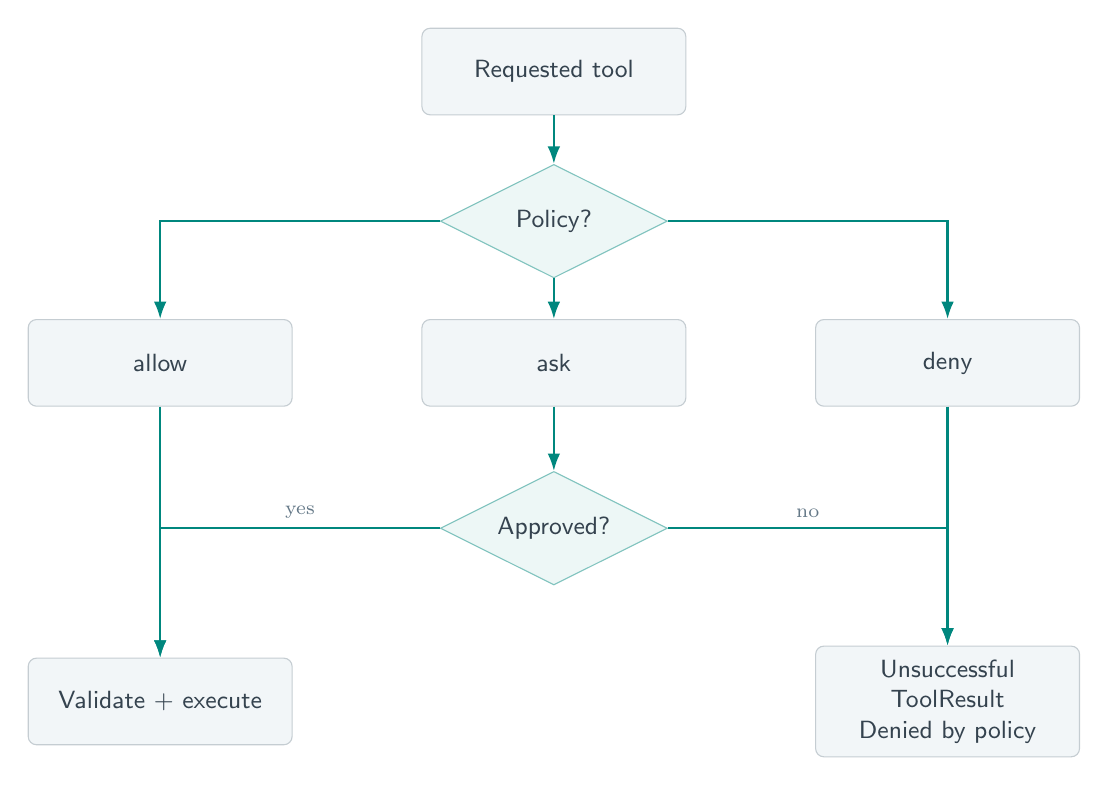
\begin{tikzpicture}
  \node[block] (request) at (0,7.2) {Requested tool};
  \node[decision] (mode) at (0,5.3) {Policy?};
  \node[block] (allow) at (-5,3.5) {allow};
  \node[block] (ask) at (0,3.5) {ask};
  \node[block] (deny) at (5,3.5) {deny};
  \node[decision] (person) at (0,1.4) {Approved?};
  \node[block] (execute) at (-5,-.8) {Validate + execute};
  \node[block] (error) at (5,-.8) {Unsuccessful ToolResult\\Denied by policy};
  \draw[arrow] (request)--(mode);
  \draw[arrow] (mode.west)-|(allow.north);
  \draw[arrow] (mode)--(ask);
  \draw[arrow] (mode.east)-|(deny.north);
  \draw[arrow] (ask)--(person);
  \draw[arrow] (allow)--(execute);
  \draw[arrow] (deny)--(error);
  \draw[arrow] (person.west)-|node[above,pos=.25,font=\scriptsize,text=Muted]{yes}(execute.north);
  \draw[arrow] (person.east)-|node[above,pos=.25,font=\scriptsize,text=Muted]{no}(error.north);
\end{tikzpicture}
\end{center}
\begin{tcolorbox}[warnbox]
  Risk labels describe tools; they do not enforce an extra rule. End-of-input denies an approval request.
\end{tcolorbox}
\captionline{\refcode{src/pilot/tools/base.py}{Tool.spec, ToolArgs};
  \refcode{src/pilot/permissions.py}{CliApprover.approve}.}

% PAGE 6 -- concepts 7--8. Retry timeline: 3 nodes.
\pageheading{CONCEPTS / RELIABILITY}{Controlled waiting, repeatable evidence}
\pair{
  \card{07 / Retries}{Retries repeat failed requests. Exponential backoff doubles waits; jitter randomizes them.}{Recover from 429 request quotas, 5xx server errors, or expired waits (timeouts), within bounded attempts.}{src/pilot/providers/retry.py}{post\_json}
}{
  \card{08 / Fakes}{A fake is a controlled replacement returning scripted responses.}{Repeatable tests force failures without network. MockTransport substitutes HTTP responses to test real adapters.}{src/pilot/providers/fake.py}{FakeProvider}
}
\vspace{15mm}
\tagline{RETRY TIMELINE / A DETERMINISTIC TEST EXAMPLE}
\vspace{5mm}
\begin{center}
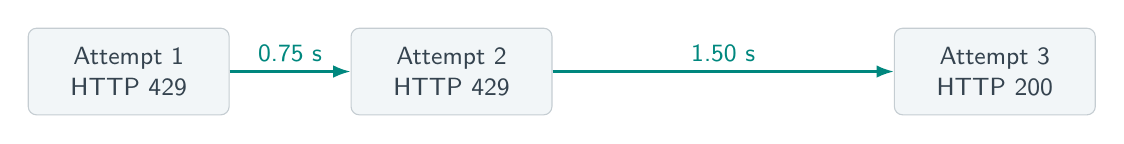
\begin{tikzpicture}
  \node[block,text width=22mm] (a) at (0,0) {Attempt 1\\HTTP 429};
  \node[block,text width=22mm] (b) at (4.1,0) {Attempt 2\\HTTP 429};
  \node[block,text width=22mm] (c) at (11,0) {Attempt 3\\HTTP 200};
  \draw[arrow] (a)--node[above,font=\sffamily\small,text=Accent]{0.75 s}(b);
  \draw[arrow] (b)--node[above,font=\sffamily\small,text=Accent]{1.50 s}(c);
\end{tikzpicture}
\end{center}
\vspace{8mm}
\begin{tcolorbox}[analogybox]
  \textbf{Analogy}\quad Wait before calling a busy office again.
\end{tcolorbox}
\vspace{5mm}
\begin{center}\small
\begin{tabular}{@{}p{.27\linewidth}p{.64\linewidth}@{}}
\toprule
\textbf{Retry} & 429 / 5xx / timeout \\
\midrule
\textbf{Fail immediately} & Permanent HTTP errors / connection failures \\
\textbf{Stop} & Attempts exhausted / Retry-After exceeds the wait cap \\
\bottomrule
\end{tabular}
\end{center}
\captionline{\refcode{tests/test_providers.py}{test\_retry\_status\_and\_jitter}:
  base delay 0.5 s, fixed jitter 0.5. Request durations are not shown.}

% PAGE 7 -- concepts 9--10. Event diagram: 5 nodes.
\pageheading{CONCEPTS / VISIBILITY}{Settings in, evidence out}
\pair{
  \card{09 / Config + secrets}{Configuration supplies settings. Secrets, such as API keys, require restricted disclosure.}{Environment overrides YAML, a readable settings format. SecretStr masks display; redaction masks known keys.}{src/pilot/config.py}{Config, load\_config}
}{
  \card{10 / Events + traces}{Events record occurrences. An event bus delivers them to subscribers: registered listeners.}{A trace records one run. JSONL stores one JSON object per line.}{src/pilot/events.py}{EventBus, TraceWriter}
}
\vspace{12mm}
\begin{center}
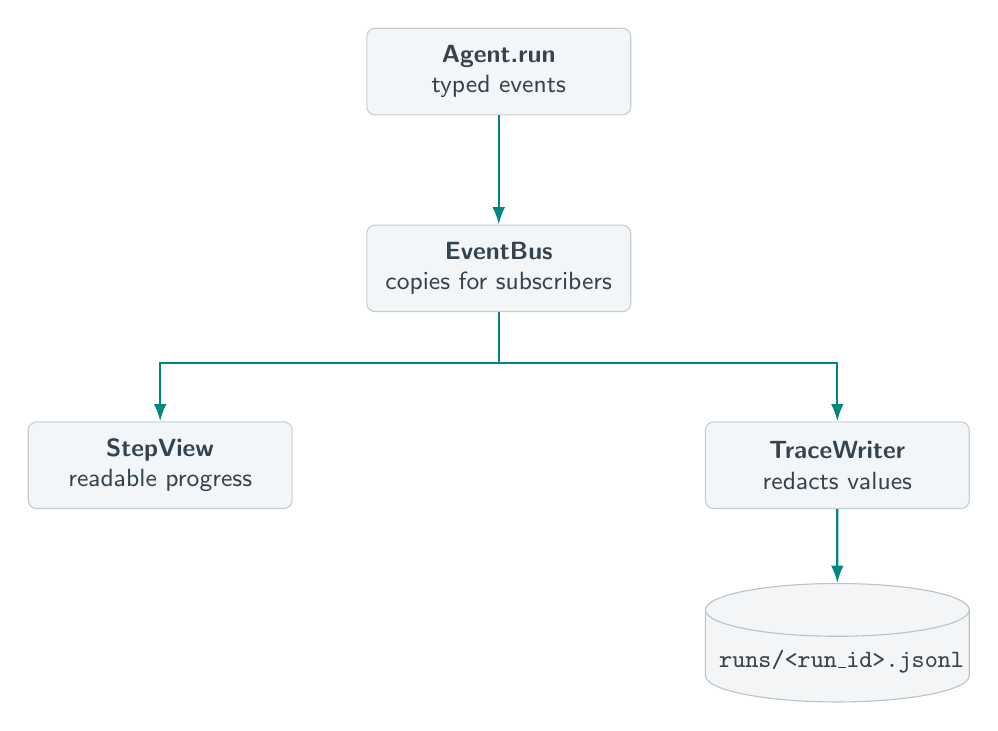
\begin{tikzpicture}
  \node[block] (agent) at (0,6.1) {\textbf{Agent.run}\\typed events};
  \node[block] (bus) at (0,3.6) {\textbf{EventBus}\\copies for subscribers};
  \node[block] (view) at (-4.3,1.1) {\textbf{StepView}\\readable progress};
  \node[block] (writer) at (4.3,1.1) {\textbf{TraceWriter}\\redacts values};
  \node[store] (file) at (4.3,-1.4) {\texttt{runs/<run\_id>.jsonl}};
  \draw[arrow] (agent)--(bus);
  \draw[arrow] (bus.south)--(0,2.4)-|(view.north);
  \draw[arrow] (bus.south)--(0,2.4)-|(writer.north);
  \draw[arrow] (writer)--(file);
\end{tikzpicture}
\end{center}
\begin{tcolorbox}[analogybox]
  \textbf{Settings precedence}\quad Provider flag\; $>$\; environment\; $>$\; .env\; $>$\; YAML\; $>$\; defaults.
\end{tcolorbox}
\captionline{Subscribers run immediately; trace-write errors stop subsequent actions.}

% PAGE 8 -- request timeline: 6 nodes.
\pageheading{WALKTHROUGH}{Follow one request}
\captionline{Existing offline scenario:
  \refcode{tests/test_cli.py}{test\_cli\_with\_real\_adapter\_and\_mock\_http}.
  No live-provider claim.}
\vspace{5mm}
\begin{center}
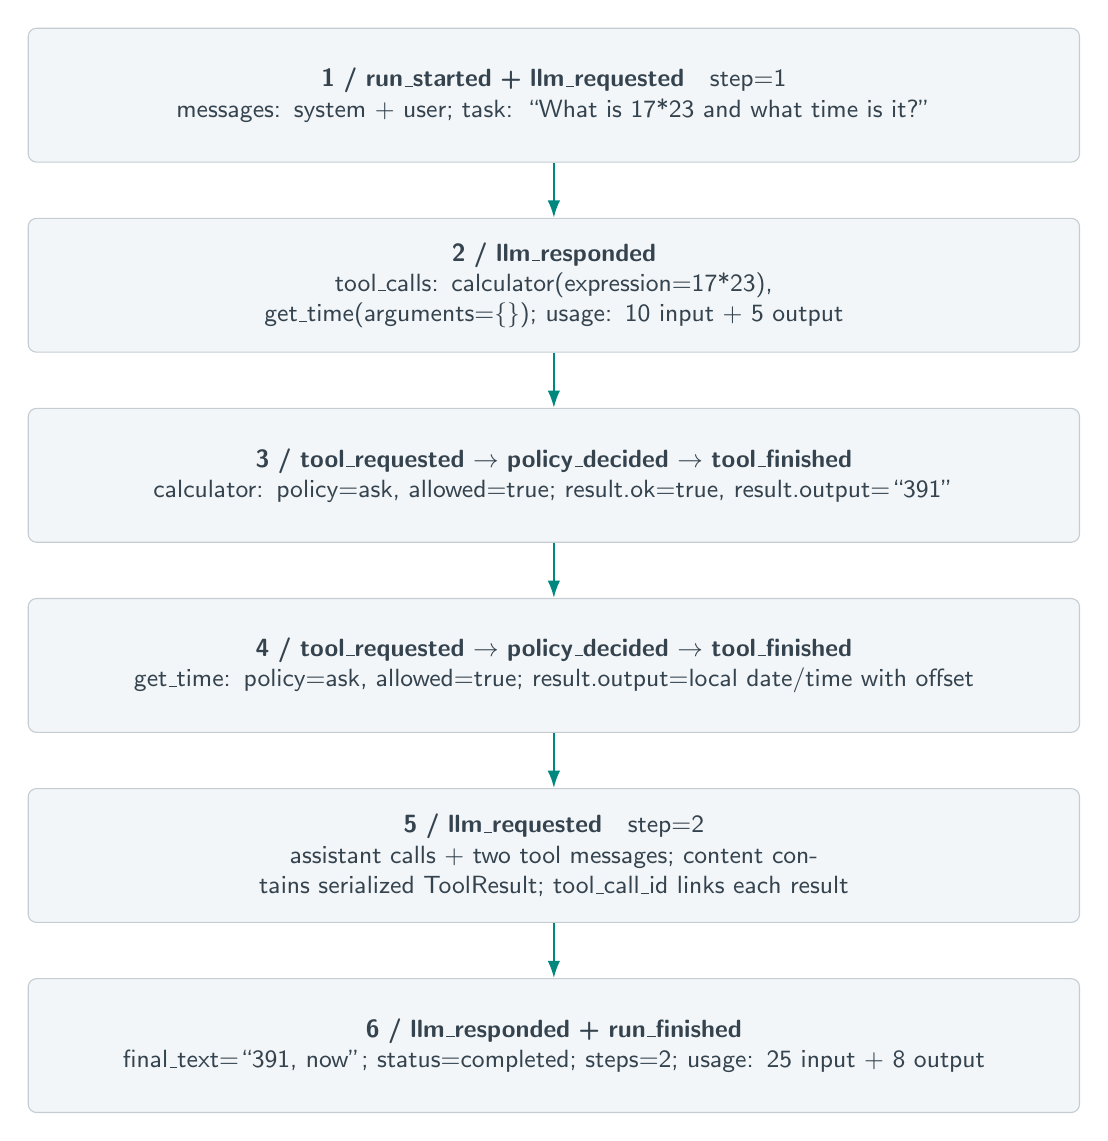
\begin{tikzpicture}[node distance=7mm]
  \node[block,text width=13cm,minimum height=17mm] (one) {
    \textbf{1 / run\_started + llm\_requested}\quad step=1\\
    messages: system + user; task: ``What is 17*23 and what time is it?''};
  \node[block,text width=13cm,minimum height=17mm,below=of one] (two) {
    \textbf{2 / llm\_responded}\\
    tool\_calls: calculator(expression=17*23), get\_time(arguments=\{\}); usage: 10 input + 5 output};
  \node[block,text width=13cm,minimum height=17mm,below=of two] (three) {
    \textbf{3 / tool\_requested $\rightarrow$ policy\_decided $\rightarrow$ tool\_finished}\\
    calculator: policy=ask, allowed=true; result.ok=true, result.output=``391''};
  \node[block,text width=13cm,minimum height=17mm,below=of three] (four) {
    \textbf{4 / tool\_requested $\rightarrow$ policy\_decided $\rightarrow$ tool\_finished}\\
    get\_time: policy=ask, allowed=true; result.output=local date/time with offset};
  \node[block,text width=13cm,minimum height=17mm,below=of four] (five) {
    \textbf{5 / llm\_requested}\quad step=2\\
    assistant calls + two tool messages; content contains serialized ToolResult; tool\_call\_id links each result};
  \node[block,text width=13cm,minimum height=17mm,below=of five] (six) {
    \textbf{6 / llm\_responded + run\_finished}\\
    final\_text=``391, now''; status=completed; steps=2; usage: 25 input + 8 output};
  \draw[arrow] (one)--(two); \draw[arrow] (two)--(three);
  \draw[arrow] (three)--(four); \draw[arrow] (four)--(five); \draw[arrow] (five)--(six);
\end{tikzpicture}
\end{center}
\vfill
\begin{tcolorbox}[conceptbox,title={Shared event fields}]
  \texttt{type / timestamp / run\_id / agent\_id / parent\_id}\par
  Here: agent\_id=pilot, parent\_id=null. Identifiers and timestamps vary.
\end{tcolorbox}
\captionline{\refcode{src/pilot/events.py}{BaseEvent};
  \refcode{src/pilot/agent/loop.py}{Agent.run}. Serialization converts structured values to text.}

% PAGE 9 -- six decisions.
\pageheading{DESIGN}{Choices and their costs}
\begin{tcolorbox}[analogybox]
  SDK means a vendor's client library. Sequential means one call at a time.
\end{tcolorbox}
\vspace{8mm}
\small
\begin{tabular}{@{}p{.19\linewidth}p{.17\linewidth}p{.29\linewidth}p{.25\linewidth}@{}}
\toprule
\textbf{Decision} & \textbf{Alternative} & \textbf{Why we chose it} & \textbf{Cost} \\
\midrule
Direct HTTP & Vendor SDK & Visible translation & Maintain formats \\[6mm]
Sequential tools & Parallel tools & Predictable approval order & No overlap \\[6mm]
Ask by default & Allow by default & Explicit human consent & Prompt fatigue \\[6mm]
Validate arguments & Trust model output & Reject malformed calls & Another exchange \\[6mm]
Reported usage & Estimate first & Provider-supplied counts & Can overshoot \\[6mm]
Synchronous bus & Separate delivery & Simple event ordering & Subscribers can stall \\
\bottomrule
\end{tabular}
\normalsize
\vfill
\begin{tcolorbox}[conceptbox,title={Read the decision against the code}]
  Simplicity reduces moving parts. It does not remove the cost shown in the last column.
\end{tcolorbox}
\captionline{\path{docs/DECISIONS.md}; \refcode{src/pilot/agent/loop.py}{Agent.run};
  \refcode{src/pilot/providers/retry.py}{post\_json}; \refcode{src/pilot/events.py}{EventBus.emit}.}

% PAGE 10 -- six failure rows.
\pageheading{OPERATIONS}{What can fail?}
\small
\begin{tabular}{@{}p{.22\linewidth}p{.73\linewidth}@{}}
\toprule
\textbf{Failure} & \textbf{Our defence / remaining gap} \\
\midrule
Endless tool loop & Step and reported-token limits.\\
 & \refcode{src/pilot/agent/loop.py}{Agent.run} \\[4mm]
Malformed request & Unknown names and invalid arguments become error results.\\
 & \refcode{src/pilot/tools/registry.py}{ToolRegistry.execute} \\[4mm]
Rate-limit storm & Bounded waits; no shared multi-agent rate controller.\\
 & \refcode{src/pilot/providers/retry.py}{post\_json} \\[4mm]
Unapproved action & Policy check precedes execution.\\
 & \refcode{src/pilot/permissions.py}{PolicyEngine.decide} \\[4mm]
Prompt injection & Untrusted text redirects a model: prompt advice only.\\
 & \refcode{src/pilot/agent/prompts.py}{DEFAULT\_SYSTEM\_PROMPT} \\[4mm]
Secret leakage & Known keys masked; arbitrary personal data is not scrubbed.\\
 & \refcode{src/pilot/events.py}{Redactor} \\
\bottomrule
\end{tabular}
\normalsize
\vfill
\begin{tcolorbox}[warnbox]
  A failed trace write can prevent the final event from being recorded.
  Closing a file is not a guarantee of recovery after a machine crash.
\end{tcolorbox}

% PAGE 11 -- five short interview answers.
\pageheading{INTERVIEW CORNER}{Explain the boundary}
\begin{tcolorbox}[interviewbox,title={What makes this an agent?}]
  It repeatedly chooses tools and observes results. Python controls whether requested actions execute.
\end{tcolorbox}
\begin{tcolorbox}[interviewbox,title={Why hide provider formats?}]
  One interface keeps orchestration independent. Adapters preserve vendor-specific formats and context.
\end{tcolorbox}
\begin{tcolorbox}[interviewbox,title={Why inject dependencies?}]
  Each instance receives its collaborators. Tests replace providers without changing the loop.
\end{tcolorbox}
\begin{tcolorbox}[interviewbox,title={Does JSON Schema make a tool safe?}]
  It describes input shape. Permission checks and tool-specific restrictions remain necessary.
\end{tcolorbox}
\begin{tcolorbox}[interviewbox,title={Why script model responses in tests?}]
  A fixed script makes failures repeatable. It cannot prove live compatibility or model judgment.
\end{tcolorbox}
\vfill
\captionline{Revisit \texttt{Agent.run}, \texttt{LLMProvider}, \texttt{ToolArgs}, and \texttt{FakeProvider} in the concept references.}

% PAGE 12 -- checklist and quiz.
\pageheading{PRACTICE}{Try it, then explain it}
\begin{tcolorbox}[analogybox]
  Set \texttt{UV\_OFFLINE=true}. These commands inspect settings or run existing offline tests.
\end{tcolorbox}
\small
\begin{itemize}[label={\textcolor{Accent}{\fbox{\rule{0pt}{.8ex}\rule{.8ex}{0pt}}}}]
  \item \textbf{Inspect settings}\par
    \texttt{uv run pilot config show}\par
    Observe: keys masked.
  \item \textbf{Change permission}\par
    \texttt{PILOT\_POLICY\_\_TOOLS\_\_CALCULATOR=deny}\par
    Prefix \texttt{uv run pilot tools}. Observe: calculator policy changes.
  \item \textbf{Lower the limit}\par
    \texttt{PILOT\_LIMITS\_\_MAX\_STEPS=1}\par
    Prefix \texttt{uv run pilot config show}. Observe: effective limit is 1.
  \item \textbf{Inspect errors}\par
    \texttt{uv run pytest -k tool\_errors\_return\_to\_model}\par
    Observe: three cases pass.
\end{itemize}
\normalsize
\vspace{5mm}
\begin{tcolorbox}[conceptbox,title={Quick quiz / answers on the last page}]
\begin{enumerate}
  \item Why resend earlier messages?
  \item Who executes a tool call?
  \item What replaces invalid arguments?
  \item Does high risk automatically deny?
  \item Can token usage overshoot?
  \item Why add retry jitter?
  \item What does a fake prove?
  \item Why can tracing stop execution?
\end{enumerate}
\end{tcolorbox}
\captionline{\refcode{tests/test_agent.py}{test\_tool\_errors\_return\_to\_model}.}

% PAGE 13 -- one-line entries in two columns.
\pageheading{REFERENCE}{Glossary at a glance}
\begin{tcolorbox}[conceptbox,title={Plain English / technical name}]
\footnotesize
\begin{minipage}[t]{.485\linewidth}
\term{Adapter}{Format translator.}
\term{Agent}{Action coordinator.}
\term{API}{Calling contract.}
\term{Backoff}{Growing waits.}
\term{Configuration}{Operating settings.}
\term{Dependency}{Required collaborator.}
\term{Dependency injection}{Explicit collaborators.}
\term{Event}{Recorded occurrence.}
\term{Event bus}{Subscriber dispatcher.}
\term{Fake}{Controlled replacement.}
\term{Global state}{Shared mutable data.}
\term{Guardrail}{Execution boundary.}
\term{HTTP}{Web request protocol.}
\term{Human-in-the-loop}{Person decides.}
\term{Interface}{Required behavior.}
\term{Jitter}{Random wait variation.}
\term{JSON}{Structured text.}
\term{JSON Schema}{Data-shape rules.}
\term{JSONL}{One JSON per line.}
\term{Least privilege}{Minimum access.}
\end{minipage}\hfill
\begin{minipage}[t]{.485\linewidth}
\term{LLM}{Language generator.}
\term{Message role}{Source/purpose label.}
\term{MockTransport}{Substituted HTTP responses.}
\term{Policy}{Allow/ask/deny rule.}
\term{Protocol}{Python interface contract.}
\term{Provider}{Model service.}
\term{Pydantic}{Data-validation library.}
\term{Rate limit}{Request quota.}
\term{Redaction}{Secret masking.}
\term{REST}{HTTP API style.}
\term{Schema}{Expected data structure.}
\term{SDK}{Vendor client library.}
\term{Secret}{Sensitive value.}
\term{Serialization}{Values to text.}
\term{Stateless}{No automatic memory.}
\term{Subscriber}{Event listener.}
\term{Synchronous}{Calls in sequence.}
\term{Timeout}{Waiting deadline.}
\term{Token}{Model counting unit.}
\term{Trace}{Run history.}
\term{UTC}{Reference time.}
\term{Validation}{Input checks.}
\term{YAML}{Readable configuration.}
\end{minipage}
\end{tcolorbox}
\vfill
\captionline{Symbols keep their Python names; glossary definitions describe their role rather than individual code lines.}

% PAGE 14 -- teaser first, compact answers last.
\pageheading{LOOK AHEAD}{The next boundary}
\begin{tcolorbox}[conceptbox,title={Next phase / scope to be defined}]
  Add one narrowly permissioned capability.\\
  Define accepted inputs and external effects first.\\
  Reuse these interfaces; test failures and denials.
\end{tcolorbox}
\vfill
\begin{tcolorbox}[interviewbox,title={Answers / quick quiz}]
\small
\begin{enumerate}
  \item Each stateless request needs its context explicitly.
  \item Python, after policy and validation.
  \item An unsuccessful ToolResult, returned to the model.
  \item No. Configured policy determines access.
  \item Yes. Reported usage arrives after generation.
  \item To spread requests rather than synchronize bursts.
  \item Repeatable local behavior, not live compatibility.
  \item Subscriber errors propagate before the next action.
\end{enumerate}
\end{tcolorbox}
\captionline{No planner, child agents, laptop tools, or saved conversation memory exist in this phase.}

\end{document}
